
\section{Additional information}
\label{ap:age} 

\begin{figure}[h!]
  \centering
  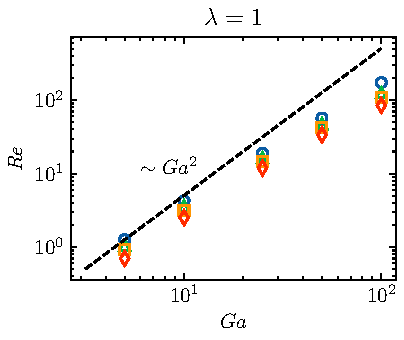
\includegraphics[height = 0.3\textwidth]{image/HOMOGENEOUS_NEW/CA/Re_l_1.pdf}
  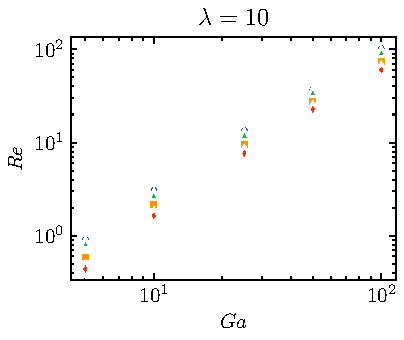
\includegraphics[height = 0.3\textwidth]{image/HOMOGENEOUS_NEW/CA/Re_l_10.pdf}
  \caption{
      Averaged Reynolds number based on the averaged drift velocity, $Re = \rho_fU d /\mu_f$, with $U = |\textbf{u}_p - \textbf{u}_f|$.
      $\textbf{u}_p$ and $\textbf{u}_f$ are the particle and fluid phase volume and time averaged velocity.
  }
  \label{fig:Reall}
\end{figure}

\begin{table}  
\begin{tabular}{c|c|c|c|l}
  calls  &  total  &   self  & \% total  & function \\ \hline
  10636901 &  4861.39 &  4861.39  &   31.8\% (28.4\% - 36.7\%) &   mpi\_boundary\_level():grid/multigrid-mpi.h:83\\
     53604 &  3097.64 &  1988.97  &   13.0\% (10.8\% - 14.7\%) &   project():poisson.h:501\\
     26802 &  2022.99 &  1236.57  &    8.1\% ( 7.3\% -  8.8\%) &   viscosity():viscosity.h:173\\
    107208 &  1984.59 &  1223.33  &    8.0\% ( 6.9\% -  8.9\%) &   heights():heights.h:281\\
     26802 &  2499.81 &  1099.66  &    7.2\% ( 6.1\% -  7.9\%) &   vof\_0():vof.h:365\\
   3155070 &  983.66  & 983.66    &  6.4\% ( 3.9\% -  9.1\%)   & mpi\_all\_reduce0():common.h:683\\
     26802 &  2372.23 &  896.09   &   5.9\% ( 5.1\% -  6.5\%)  &  advection\_term():navier-stokes/centered.h:323\\
     26802 &  1583.59 &  645.89   &   4.2\% ( 4.1\% -  4.3\%)  &  no\_coalescence():./no-coalescence.h:419\\
      2681 &  584.39  & 372.15    &  2.4\% ( 2.4\% -  2.5\%)   & track\_bub():RS.c:124\\
    321624 &  546.74  & 340.36    &  2.2\% ( 1.8\% -  2.6\%)   & reconstruction():fractions.h:476\\
    107208 &  2777.30 &  303.23   &   2.0\% ( 1.6\% -  2.4\%)  &  curvature():curvature.h:621\\
     69275 &  992.44  & 254.14    &  1.7\% ( 1.4\% -  1.8\%)   & tag():tag.h:268\\
     26802 &  328.67  & 202.85    &  1.3\% ( 1.1\% -  1.5\%)   & acceleration\_0():iforce.h:133\\
     26802 &  2257.27 &  178.19   &   1.2\% ( 0.8\% -  1.3\%)  &  projection():navier-stokes/centered.h:430\\
  %    26802 &  2142.30 &  119.30   &   0.8\% ( 0.5\% -  0.9\%)  &  viscous\_term():navier-stokes/centered.h:362\\
  %    26802 &  145.95  & 116.09    &  0.8\% ( 0.5\% -  0.9\%)   & acceleration\_2():RS.c:166\\
  %    26803 &  111.60  & 111.57    &  0.7\% ( 0.5\% -  0.8\%)   & properties\_0():two-phase-generic.h:101\\
  %    26802 &  172.09  & 100.18    &  0.7\% ( 0.5\% -  0.8\%)   & acceleration():navier-stokes/centered.h:386\\
  %    69275 &   68.91  &  68.88    &  0.5\% ( 0.4\% -  0.5\%)   & z\_indexing():grid/multigrid-mpi.h:145\\
  %      118 &   59.59  &  59.59    &  0.4\% ( 0.2\% -  0.8\%)   & compose\_image():view.h:409\\
  %    26802 &   64.69  &  34.48    &  0.2\% ( 0.2\% -  0.3\%)   & tracer\_advection\_1():./no-coalescence.h:446\\
  %       59 &  129.57  &  28.81    &  0.2\% ( 0.1\% -  0.2\%)   & movies():RS.c:244\\
  %    26803 &   92.48  &  27.24    &  0.2\% ( 0.1\% -  0.2\%)   & stability\_1():tension.h:64\\
  %    26803 &   24.42  &  21.33    &  0.1\% ( 0.1\% -  0.1\%)   & stability():navier-stokes/centered.h:226\\
  % 43894361 &  3001.24 &    5.50   &   0.0\% ( 0.0\% -  0.0\%)  &  boundary\_internal():grid/cartesian-common.h:450\\
  % 42061052 &   25.50  &   3.61    &  0.0\% ( 0.0\% -  0.0\%)   & interpolate():grid/cartesian-common.h:815\\
  %      472 &    2.31  &   2.31    &  0.0\% ( 0.0\% -  0.0\%)   & draw\_vof():draw.h:1052\\
  %    58554 &   25.92  &   0.87    &  0.0\% ( 0.0\% -  0.0\%)   & reduce\_bubbles():./no-coalescence.h:158\\
  %        1 &  15287.89&     0.73  &    0.0\% ( 0.0\% -  0.0\%) &   run():run.h:37\\
  %        1 &    0.28  &   0.28    &  0.0\% ( 0.0\% -  0.0\%)   & init\_0():RS.c:149\\
  %    26802 &  2777.57 &    0.27   &   0.0\% ( 0.0\% -  0.0\%)  &  acceleration\_1():tension.h:94\\
  %      236 &   38.81  &   0.21    &  0.0\% ( 0.0\% -  0.0\%)   & squares():draw.h:1375\\
    %    118 &   59.64  &   0.05    &  0.0\% ( 0.0\% -  0.1\%)   & save():view.h:529\\
    %  63404 &    0.06  &   0.03    &  0.0\% ( 0.0\% -  0.0\%)   & interpolate():grid/cartesian-common.h:816\\
    %      1 &    0.02  &   0.02    &  0.0\% ( 0.0\% -  0.0\%)   & defaults\_3():iforce.h:38\\
    %      1 &    0.01  &   0.01    &  0.0\% ( 0.0\% -  0.0\%)   & defaults\_2():two-phase-generic.h:26\\
    %  26802 &  1583.60 &    0.01   &   0.0\% ( 0.0\% -  0.0\%)  &  vof\_1():./no-coalescence.h:430\\
    %  26802 &    0.01  &   0.01    &  0.0\% ( 0.0\% -  0.0\%)   & set\_dtmax():navier-stokes/centered.h:222\\
    %  26803 &    0.00  &   0.00    &  0.0\% ( 0.0\% -  0.0\%)   & stability\_0():vof.h:143\\
    %      1 &    0.25  &   0.00    &  0.0\% ( 0.0\% -  0.0\%)   & init():navier-stokes/centered.h:213\\
    %      1 &    0.00  &   0.00    &  0.0\% ( 0.0\% -  0.0\%)   & defaults\_0():navier-stokes/centered.h:181\\
    %      1 &    0.00  &   0.00    &  0.0\% ( 0.0\% -  0.0\%)   & restore():output.h:1169\\
    %      1 &    0.00  &   0.00    &  0.0\% ( 0.0\% -  0.0\%)   & cleanup():run.h:52\\
    %      1 &    0.00  &   0.00    &  0.0\% ( 0.0\% -  0.0\%)   & defaults():run.h:44\\
    %      1 &    0.00  &   0.00    &  0.0\% ( 0.0\% -  0.0\%)   & defaults\_4():./no-coalescence.h:483\\
    %      1 &    0.00  &   0.00    &  0.0\% ( 0.0\% -  0.0\%)   & defaults\_1():vof.h:134\\
    %      1 &    0.00  &   0.00    &  0.0\% ( 0.0\% -  0.0\%)   & cleanup\_0():./no-coalescence.h:458\\
    %      1 &    0.00  &   0.00    &  0.0\% ( 0.0\% -  0.0\%)   & default\_display():navier-stokes/centered.h:188\\
    %      1 &    0.00  &   0.00    &  0.0\% ( 0.0\% -  0.0\%)   & stop():RS.c:272\\
\end{tabular}
\caption{Profiling of the time taken by functions during the simulation for the parameters.
This simulation has been carried with the Following dimensionless parameters : 
$Ga = 25$, $\lambda = 1$, $Bo = 1$, $\zeta = 1.11$ and $\phi = 0.2$.
Regarding the numerical parameters :  $N_b = 125$, $d/\Delta = 37.149$. }
\label{tab:performance}
\end{table}


\begin{figure}[h!]
    \centering
    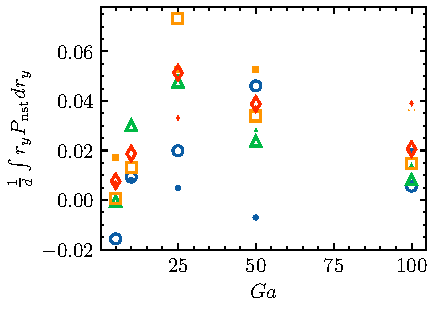
\includegraphics[height = 0.3\textwidth]{image/HOMOGENEOUS_NEW/PA/R.pdf}
    \caption{ First moment of the nearest particle pair distribution in the direction of gravity. 
    ($\pmb\bigcirc$) $\phi = 0.01$; ($\pmb\triangle$) $ \phi = 0.05$; ($\pmb\square$) $\phi = 0.1$ ($\pmb\lozenge$) $\phi = 0.2$.
    The hollow symbols correspond to $\lambda = 1$, the filled symbols to $\lambda = 10$.
    For $r<d$ we arbitrarily set $P_\text{r}^\text{th} = 1$ so that the distribution can be visualized.
    Black symbols represent the results of \citet{zhang2023evolution} for hard sphere suspension with $\phi = 0.016,0.056,0.134,0.262$  %$\phi = 0.0168,0.0565,0.1341,0.2622$ 
    corresponding to $\pmb\times,\pmb +, \pmb\star , \pmb\triangledown$, respectively.
    }
    \label{fig:ap:RY}
\end{figure}

\begin{figure}
  \centering
  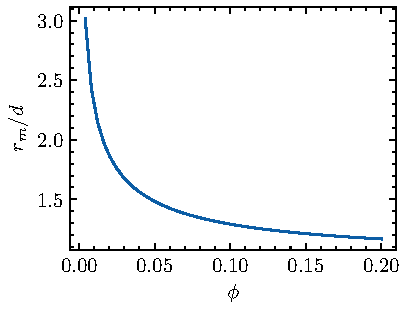
\includegraphics[height = 0.3\textwidth]{image/HOMOGENEOUS_NEW/PA/rm.pdf}
  \caption{Dimensionless radial distance to the nearest neighbor for a random distribution.}
  \label{fig:ap:agee}
\end{figure}